\chapter{Implementation}
\label{chap:implementation}

In the previous chapter, we described the theoretical background for the \emph{InterfaceSmith} programming system, defined the types representing the input data and UI elements, described operations on these types, and showcased the system's core functionality.
In this chapter, we describe the implementation according to the design principles described in Chapter~\ref{chap:design} and the data-driven UI creation described in Chapter~\ref{chap:corelogic}.
We explore the technologies chosen, the system's architecture, and key implementation details.
\medskip
\section{Technologies}
\label{sec:technologies}
To provide context for the implementation, we'll first examine the technologies used in developing the \emph{InterfaceSmith} system.

We created the \emph{InterfaceSmith} programming system as a browser-based client-side application providing a graphical user interface rather than a traditional desktop application.
The main reasons were to allow cross-platform compatibility and the ability to see the preview of the created web applications in a browser-based environment.

To implement the application, we employed various existing tools that aligned with our vision for the application and fulfilled our demands on the functionality they provide.
We wanted to implement the system using a programming language with functional programming capabilities and a strong ecosystem, which narrowed our range of suitable options and subsequently influenced which supplementary technologies we could use.
The system is implemented using the following key technologies:
\begin{itemize}
	\item \textbf{F\#:} The \citet{fsharp} programming language is used to implement the entire application, including the core logic and the user interface, chosen for its strong type system and functional programming capabilities.
	\item \textbf{Fable:} The \citet{fable} compiler, briefly described in Section~\ref{sub:Fable}, compiles the F\# source code to JavaScript, enabling browser-based execution and using technologies from the JavaScript ecosystem.
	\item \textbf{React:} The \citet{feliz} library provides a domain-specific language (DSL) for building \emph{React} user interface components and applications in F\#.
	\item \textbf{Elmish:} \citet{elmish} is a library used to enable the creation of Elmish style applications in F\#, which follow the MVU pattern described in Section~\ref{sub:elmish}.
	\item \textbf{Tailwind:} We use the Tailwind CSS framework for the layout and styling of the UI components of the application, which provides composable CSS classes and enables high customizability of the UI elements.
	\item \textbf{SimpleJson:} The \citet{simpleJson} library is used to parse the input JSON data into the internal representation described in Section~\ref{sub:json}.
	\item \textbf{SAFE stack template:} We use the \citet{safestack} template's \emph{Build} project, which provides scripts for building web applications built in F\#.
\end{itemize}

\medskip
\subsection{Alternatives}
While we selected the technologies mentioned in the previous Section for our implementation, for several of them, we considered using alternative technologies:
\begin{itemize}
	\item \textbf{Programming Language:} Instead of F\#, we could have used other programming languages such as Haskell, OCaml, or TypeScript, which also offer strong type systems and functional programming capabilities.
	      However, F\# was chosen for its seamless integration with the .NET ecosystem, high-quality development tools and documentation, and its ability to be compiled to JavaScript via Fable.
	\item \textbf{CSS Framework:} We considered using alternative CSS frameworks, such as Bulma or Bootstrap, which provide pre-made styled components.
	      We chose Tailwind instead, as the composable styling classes allow for a more direct approach to styling UI elements instead of trying to adapt and modify the pre-made components.
	\item \textbf{JSON Parsing:} Instead of Fable.SimpleJson, we could have used the closest alternative library called \citet{thoth}.
	      The main strength of this library is the ability to create custom JSON \emph{encoders} and \emph{decoders}.
	      However, as we need the ability to parse JSON data of arbitrary structure, SimpleJson's lightweight nature and its internal representation of the parsed data made it our preferred choice.
\end{itemize}
While these alternatives have their strengths, our chosen technologies provided the best balance of functional programming capabilities, browser compatibility, and ecosystem support for our specific requirements.
\medskip
\section{System architecture}
\label{sec:appArch}
Before we describe the implementation specifics, we must first describe the \emph{architecture} of the implementation.
As the main goal of the system is to allow users to create web applications based on concrete value, we decided that our main implementation unit will be a \emph{Page}, which comprises data, UI elements and custom functionality.
We see the definition of the \emph{Page} in Program~\ref{prog:page}.

The application follows a nested Elmish architecture approach.
The main application is implemented as an Elmish application responsible for the general functionality, such as Page creation, deletion, and state management across all pages.
Within this main application, each individual Page is managed by its own Elmish \emph{PageEditor} sub-application.
This provides clear separation of concerns, as the main application focuses on the management of all Pages and holds the state for all of the PageEditor sub-applications,
each PageEditor sub-application independently handles the modification of its individual Page.

\begin{listing}[H]
	\caption{The Page type definition}
	\label{prog:page}
	\begin{lstlisting}
type Page = {
    Name: string
    Id: Guid
    ParsedJson: Json
    CurrentTree: RenderingCode
    JsonString: string
    UserMessages: UserMessage list
    UpdateFunction: UpdateFunction
    CustomFunctions: Map<string, Javascript>
}
  \end{lstlisting}
\end{listing}

\medskip
\subsubsection{Main Elmish application}
At the top level, our application follows the Elm architecture described in Section~\ref{sub:elmish}.
The primary application state is represented by the \emph{Model} type, and we define corresponding \emph{view} and \emph{update} functions to manage this state.

We can see the \emph{Model} type representing the entire main application's state in Program~\ref{fig:appmodel}.
It consists of a collection of created pages, collection to store the ordering of the pages based on when they are created, the id of the currently open Page, and a variable of wheter the sidebar menu is open.

The \emph{Update} function updates the state based on a \emph{Message} it recieves and we see the \emph{Msg} type defined in Program~\ref{fig:appMsg}.
The messages represent events such as creating a new page or toggling the sidebar menu, or updating the state of a certain Page Editor.

The \emph{View} function renders the main general application elements, aswell as the Page Editor application for the selected page.
We use the \citet{feliz} library to create \emph{React} components and style them using \citet{tailwind}.

\begin{listing}[htbp]
	\caption{Definition of the Main Elmish application's Model.}
	\label{fig:appmodel}
	\begin{lstlisting}
type Model = {
    Pages: Map<Guid, PageEditorModel>
    PageOrder: Guid list
    ActivePageId: Guid option
    IsSidebarOpen: bool
}
    \end{lstlisting}
\end{listing}

\begin{listing}[htbp]
	\caption{Definition of the Main Elmish application's Msg type.}
	\label{fig:appMsg}
	\begin{lstlisting}
type Msg =
    | CreatePage
    | UpdatePage of PageEditorModel
    | DeletePage of Guid
    | ToggleSidebar
    | OpenPage of Guid
    | PageEditorMsg of Guid * PageEditorMsg
    \end{lstlisting}
\end{listing}
\medskip
\subsubsection{PageEditor sub-application}

The \emph{PageEditor} is an Elmish application that provides modification functionality for an individual Page.
It is separate from the Main application and has its own local state, update logic, and view functions while still being nested in the Main application.
It provides the functionality described in Chapter~\ref{chap:design} and Chapter~\ref{chap:corelogic}.
The state of the application is represented by the \emph{PageEditorModel}, and we define a corresponding \emph{PageEditorView} React component and the \emph{pageEditorUpdate} function to manage its state.

The \emph{PageEditorView} is implemented as a React functional component using the Feliz DSL.
The UI is inspired by the \citet{darklang} programming system and features a movable canvas containing draggable elements.
We describe the UI elements in greater detail in the following sections.

We see the \emph{PageEditorModel} representing the state of the PageEditor application in Program~\ref{fig:editorModel}.
It consists of the specific \emph{Page}, types for rendering the UI elements of the editor, and types for rendering the movable canvas and its elements.

The \emph{pageEditorUpdate} function updates the state based on the \emph{PageEditorMsg} dispatched by the \emph{PageEditorView}.
The main categories of the PageEditor messages are:
\begin{itemize}
	\item Input/Output operations, such as handling file upload and download events.
	\item Interactions with the PageEditor UI that do not change the state of the \emph{Page}.
	\item Modification the Page's RenderingCode AST.
	\item Modification of the Page's custom functions.
	\item Modification of the Page's Elmish-style messages.
\end{itemize}


\begin{listing}[htbp]
	\caption{The PageEditorModel type representing the state a PageEditor application.}
	\label{fig:editorModel}
	\begin{lstlisting}
type PageEditorModel = {
    PageData: Page
    FileUploadError: bool
    ViewportPosition: Position
    Scale: float
    Elements: Element list
    DraggingElementId: int option
    IsPanning: bool
    LastMousePosition: Position option
    IsPreviewOpen: bool
    ContextMenuVisible: bool
    ContextMenuPosition: Position option
}    
  \end{lstlisting}
\end{listing}
\medskip
\subsection{Module structure}
\nopagebreak[4]
The implementation is divided between different F\# \emph{modules}, each providing different functionality.
We define two main modules named \emph{Core Logic} and \emph{Editor}, which contain sub-modules implementing specific functionality.
These modules can be described as follows:
\begin{enumerate}
	\item \textbf{Core Logic module:} Contains modules responsible for implementing the Core logic described in Chapter~\ref{chap:corelogic}, such as the representation of the UI elements and the various operations on these types.
	\item \textbf{Editor module:} Modules focused on implementing the user interface of the programming system and its functionality following the Elm architecture described in Section~\ref{sub:elmish}.
	      The modules use and depend on the functionality provided by the CoreLogic module.
\end{enumerate}

Each sub-module comprises various functions or type definitions.
In our implementation, we separate type definitions and functions into distinct modules, similarly to the separation of \emph{Domain} and \emph{Infrastructure} layers of the \emph{Domain-driven} architecture.
The modules containing the type definitions define the system's domain and have either none or a small number of external dependencies.
The modules containing the functions implement the behaviors and operations that manipulate and utilize the domain types.
This approach inherently makes the application more easily extensible.
For example, we can add new functionality to the Editor module without changing the domain model or the implementation of the Core Logic submodules.
\medskip
\subsubsection{Core Logic Module}
The Core Logic module is the first main module of the \emph{InterfaceSmith's} implementation.
It contains the implementation of the types and operations described in Chapter~\ref{chap:corelogic}.
Figure~\ref{fig:core-logic-structure} illustrates the overall structure of this module.
We divide the implementation into the following sub-modules:
\nopagebreak[4]
\begin{itemize}
	\item \textbf{Types:} This module comprises sub-modules that define the fundamental data structures of our system:
	      \begin{itemize}
		      \item \textbf{RenderingTypes:} Contains definitions for types such as the \emph{RenderingCode}, \emph{InnerValue}, and other related types.
	      \end{itemize}

	\item \textbf{Operations:} This module includes sub-modules that implement various operations on the types defined in the Types module:
	      \begin{itemize}
		      \item \textbf{RenderingCode:} Implements operations such as the \emph{replace} function, which modifies the RenderingCode AST.


		      \item \textbf{DataRecognition:}  Handles the mapping process between input data and our internal UI element representation.
		            It includes the \emph{recognizeJson} function, detailed in Section~\ref{sec:mapping}.

		      \item\textbf{CodeGeneration:} Provides functionality to generate textual representations of created web applications from RenderingCode ASTs.
		            Our implementation generates an MVU-style application in pure JavaScript, which we describe in the following sections.
	      \end{itemize}
\end{itemize}

\begin{figure}[H]
	\centering
	\begin{tikzpicture}[
			node distance = 0.5cm and 0.5cm,
			mainblock/.style = {rectangle, draw, fill=gray!20,
					text width=6em, text centered, rounded corners, minimum height=3em},
			typeblock/.style = {rectangle, draw, fill=blue!20,
					text width=6em, text centered, rounded corners, minimum height=3em},
			opblock/.style = {rectangle, draw, fill=green!20,
					text width=6em, text centered, rounded corners, minimum height=3em},
			line/.style = {draw, -stealth},
		]
		% Main Core Logic node
		\node [mainblock, text width=10em] (core) {Core Logic};

		% Types
		\node [typeblock, below left=of core] (types) {Types};
		\node [opblock, below=of types] (renderingtypes) {Rendering\\Types};

		% Operations
		\node [typeblock, below right=of core] (operations) {Operations};
		\node [opblock, below left=of operations] (rendering) {Rendering\\Code};
		\node [opblock, below=of operations] (recognition) {Data\\Recognition};
		\node [opblock, below right=of operations] (generation) {Code\\Generation};

		% Draw arrows
		\path [line] (core) -- (types);
		\path [line] (core) -- (operations);
		\path [line] (types) -- (renderingtypes);
		\path [line] (operations) -- (rendering);
		\path [line] (operations) -- (recognition);
		\path [line] (operations) -- (generation);


	\end{tikzpicture}
	\caption{Core Logic Module Structure}
	\label{fig:core-logic-structure}
\end{figure}
\medskip
\subsubsection{Editor module}
The Editor module is the second main module of the \emph{Data-driven UI's} implementation.
It is responsible for implementing the~programming system's UI, state management, and functionality.

As our main implementation unit, we selected a
Figure~\ref{fig:editor-module-structure} illustrates the module's structure, and we describe the implementation in greater detail in the following sections.
We divide the module into the following sub-modules:
\begin{itemize}
	\item \textbf{Types:} This module defines the core data structures that represent the state and operations of our Elmish-style application, as detailed in Section~\ref{sub:elmish}.
	      \begin{itemize}
		      \item \textbf{EditorDomain:} Definition of the domain types that represent the internal state of the entire application.
		      \item \textbf{PageEditorDomain:} Defines specialized domain types focused on representing the \emph{Page Editor} elmish-style sub-application.
	      \end{itemize}

	\item \textbf{Utilities:} Provides a collection of helper functions that support various aspects of the application:
	      \begin{itemize}
		      \item \textbf{Icons:}Icon importing and management.
		      \item \textbf{FileUpload:}File Upload handling and processing.
		      \item \textbf{JsonParsing:}JSON data parsing and serialization, leveraging the \citet{simpleJson} library.
		      \item \textbf{JavaScriptEditor:}Importing the libraries necessary to use the Codemirror editor component.
	      \end{itemize}


	\item \textbf{Components:} Implements custom components that form the interactive user interface of the Page Editor sub-applications:
	      \begin{itemize}
		      \item \textbf{ElementComponents:} Implementation of the draggable canvas elements.
		      \item \textbf{OptionsComponents:} Provides components serving as context menus to allow editing functionality for the individual RenderingCode elements.
		      \item \textbf{EditorComponents:} Provides a set of components that deliver general editor functionality, such as a collapsable side menu showing the created pages.
		      \item \textbf{PageEditorComponents:} Implements the \emph{Page Editor} elmish-style sub-application used for editing a \emph{Page}.
	      \end{itemize}
	\item \textbf{CustomRendering:} Implements dynamically rendering previews of the RenderingCode AST, together with interactive modification menus, and the rendering of the canvas elements.
\end{itemize}


\begin{figure}[H]
	\centering
	\begin{tikzpicture}[
			node distance = 1cm,
			mainblock/.style = {rectangle, draw, fill=gray!20,
					text width=8em, text centered, rounded corners, minimum height=3em},
			subblock/.style = {rectangle, draw, fill=blue!20,
					text width=7em, text centered, rounded corners, minimum height=2.5em},
			subsubblock/.style = {rectangle, draw, fill=green!20,
					text width=6em, text centered, rounded corners, minimum height=2em},
			line/.style = {draw, -stealth},
		]
		% Main Editor Module node
		\node [mainblock] (editor) {Editor Module};

		% Main sub-modules

		\node [subblock, below=of editor] (utilities) {Utilities};
		\node [subblock, left=of utilities] (types) {Types};
		\node [subblock, right=of utilities] (components) {Components};
		\node [subblock, right=of editor] (rendering) {CustomRendering};
		% Draw arrows
		\foreach \i in {types,utilities,components, rendering}
		\path [line] (editor) -- (\i);

	\end{tikzpicture}
	\caption{Editor Module Structure}
	\label{fig:editor-module-structure}
\end{figure}
\medskip
\section{Main Features}
\label{sec:features}
Now that we have defined the implementation's modular architecture and structure, we can describe the specifics of the implementation.
As the implementation comprises many different type definitions and functions of various complexity,
we will briefly describe the system's \emph{main features} that implement the design principles described in Chapter~\ref{chap:design}.

To implement the programming system, we use tools and technologies previously described in Section~\ref{sec:technologies}.
One of these tools is the \citet{feliz} library, used for creating composable \emph{React} UI components in F\#.
Another important tool is the \citet{elmish} library, which provides abstractions that enable the creation of \emph{Elm-style} applications in F\#.

\medskip
\subsection{User Interface implementation}
The integral component of our programming system is the low-code user interface, as it realizes the design principles described in Chapter~\ref{chap:design}.
It provides tools for creation and modification of UI elements through the use of context menus, shows the preview of the already created UI elements, and allows customization of the functionality of the created UI elements.
The user interface is composed of multiple React components some managed by the top-level Elmish application, while others managed by the individual PageEditor sub-applications.

\begin{figure}[H]
	\centering
	\includegraphics[width=1\linewidth]{img/UIExample.pdf}
	\caption{Example of \emph{Data-driven UI's} user interface}
	\label{fig:ui}
\end{figure}

We see the layout of the \emph{Data-driven UI's} interface in Figure~\ref{fig:ui}.
Located on the left is a collapsible side-menu used to open and delete pages, and a button to create a new page.
Users can also customize the name of the individual page, by clicking twice on the page option.
The menu is implemented as a \emph{React component}, and dispatches different messages to the \emph{update} function based on the interactions with the UI.
The state and operations of this menu is managed by the main Elmish application.

To the right side of the menu we see the movable canvas, displaying canvas elements for the selected page.
On the top of the canvas we can see a panel with three buttons, the first one is used to upload the input data for the page, the second one is used to download the generated JavaScript source code for the created page,
and the third button is used to preview the generated JavaScript code for the page.
The canvas elements are draggable and some are also resizable.
The state and operations of the canvas and its content is managed by the individual PageEditor applications.

\subsubsection{Canvas elements}
\begin{itemize}
	\item \textbf{ModelElement:} Displays the uploaded data. Each field is collapsible and also shows the type of the field. We an example of this element in Figure~\ref{fig:model-menu}.
	      \begin{figure}[htbp]
		      \begin{center}
			      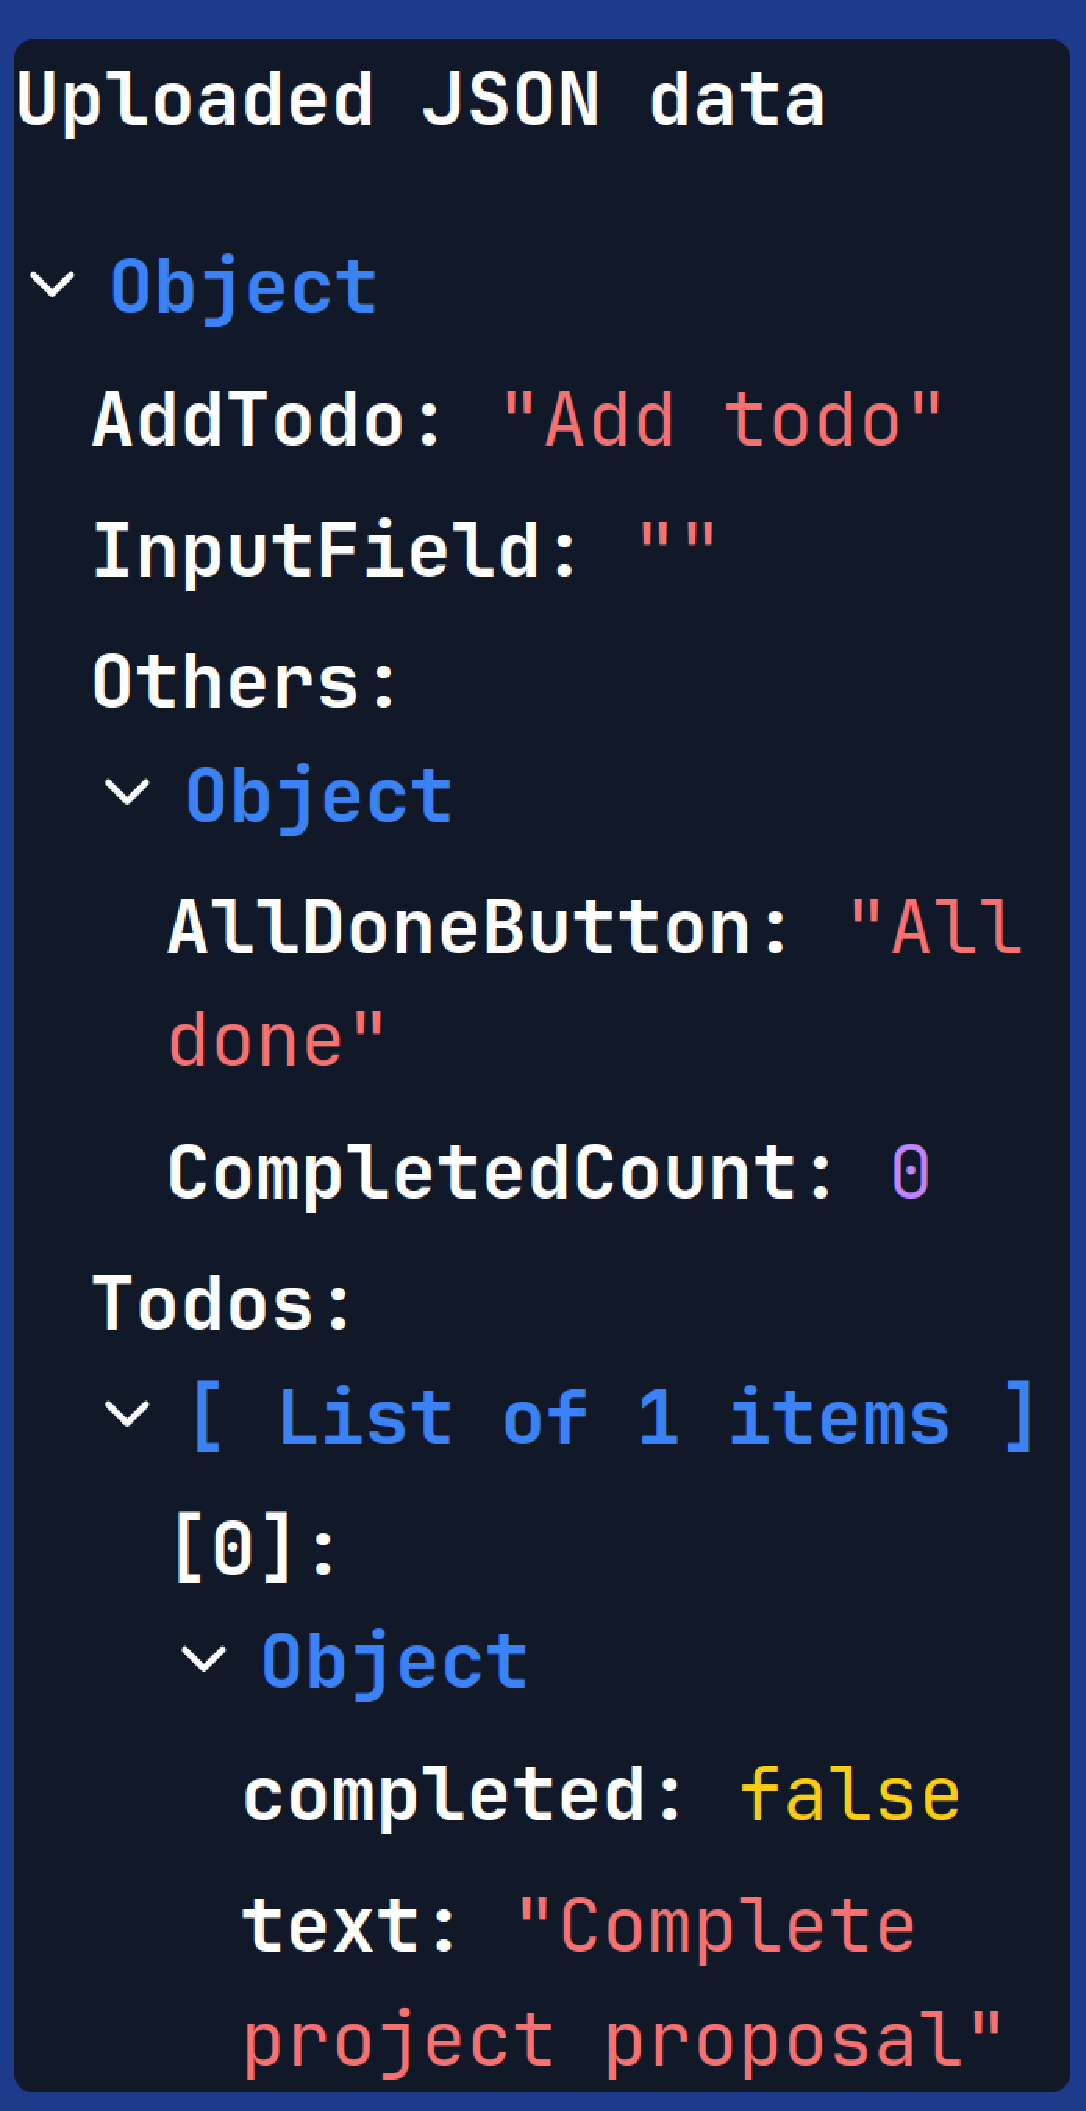
\includegraphics[width=0.35\textwidth]{img/json-menu.pdf}
		      \end{center}
		      \caption{The canvas ModelElement showing a preview of the uploaded JSON data.}\label{fig:model-menu}
	      \end{figure}

	\item \textbf{FunctionsElement:} Provides options to create, delete and modify custom functions. It also provides an editor window to write the function implementation. We see the element displayed in Figure~\ref{fig:functions-menu}.
	      \begin{figure}[htbp]
		      \begin{center}
			      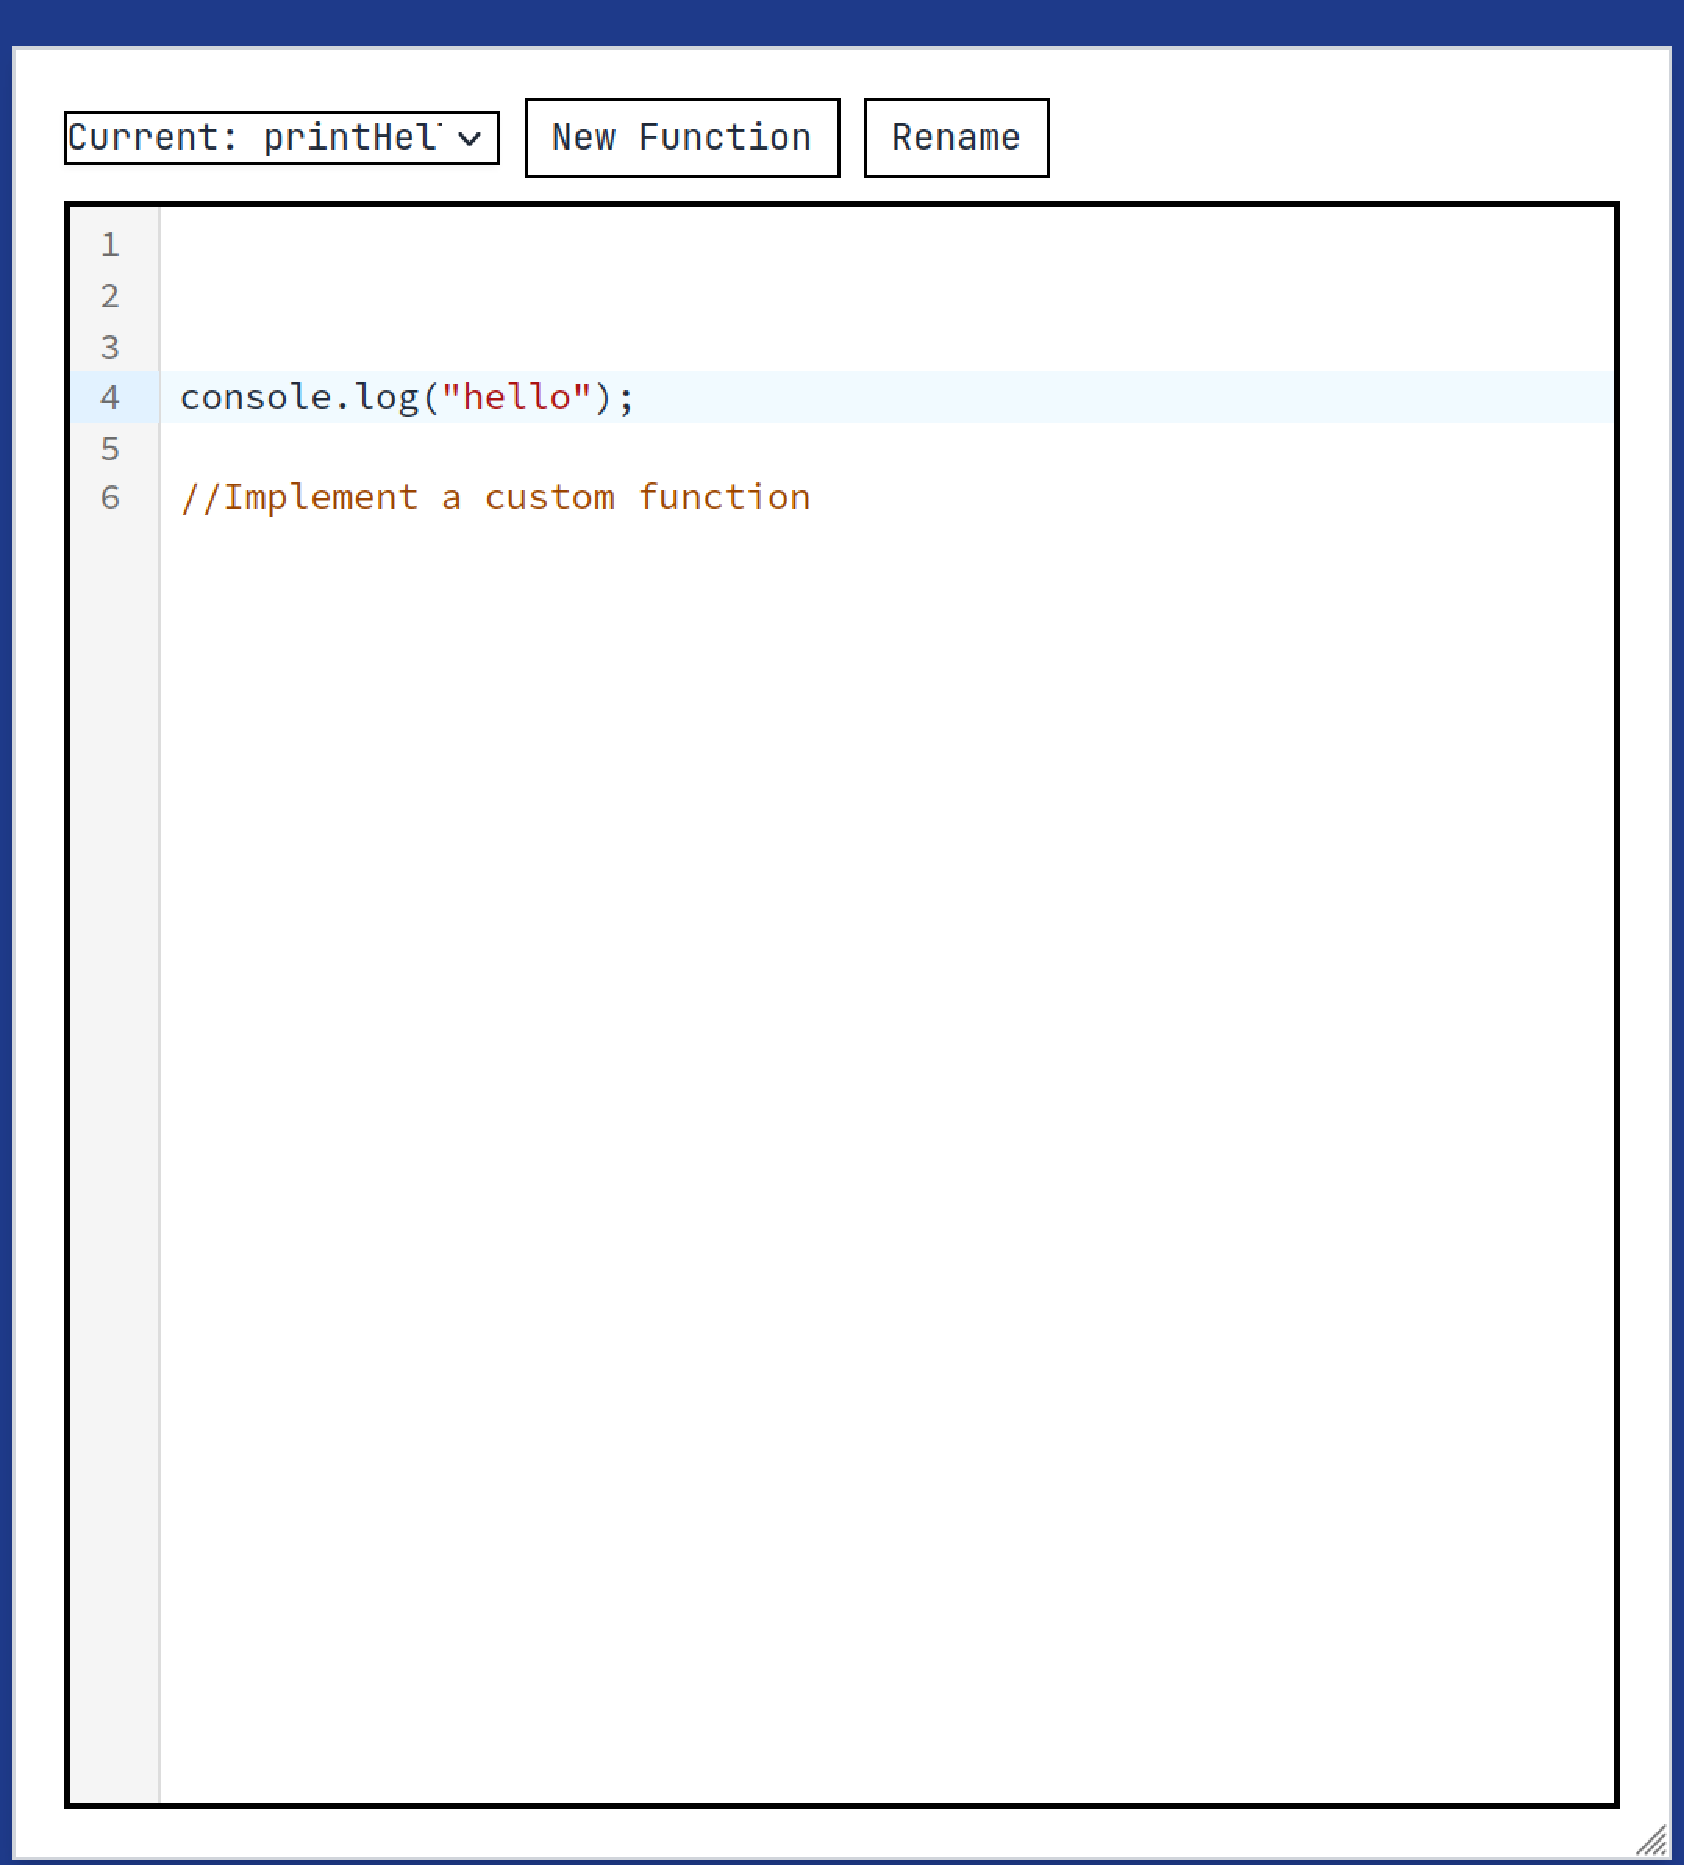
\includegraphics[width=0.7\textwidth]{img/function-menu.pdf}
		      \end{center}
		      \caption{The canvas FunctionsElement }\label{fig:functions-menu}
	      \end{figure}
	\item \textbf{MessageAndUpdateElement:} Allows the user to create new messages and modify the update function's modification of the model.
	      \begin{figure}[htbp]
		      \begin{center}
			      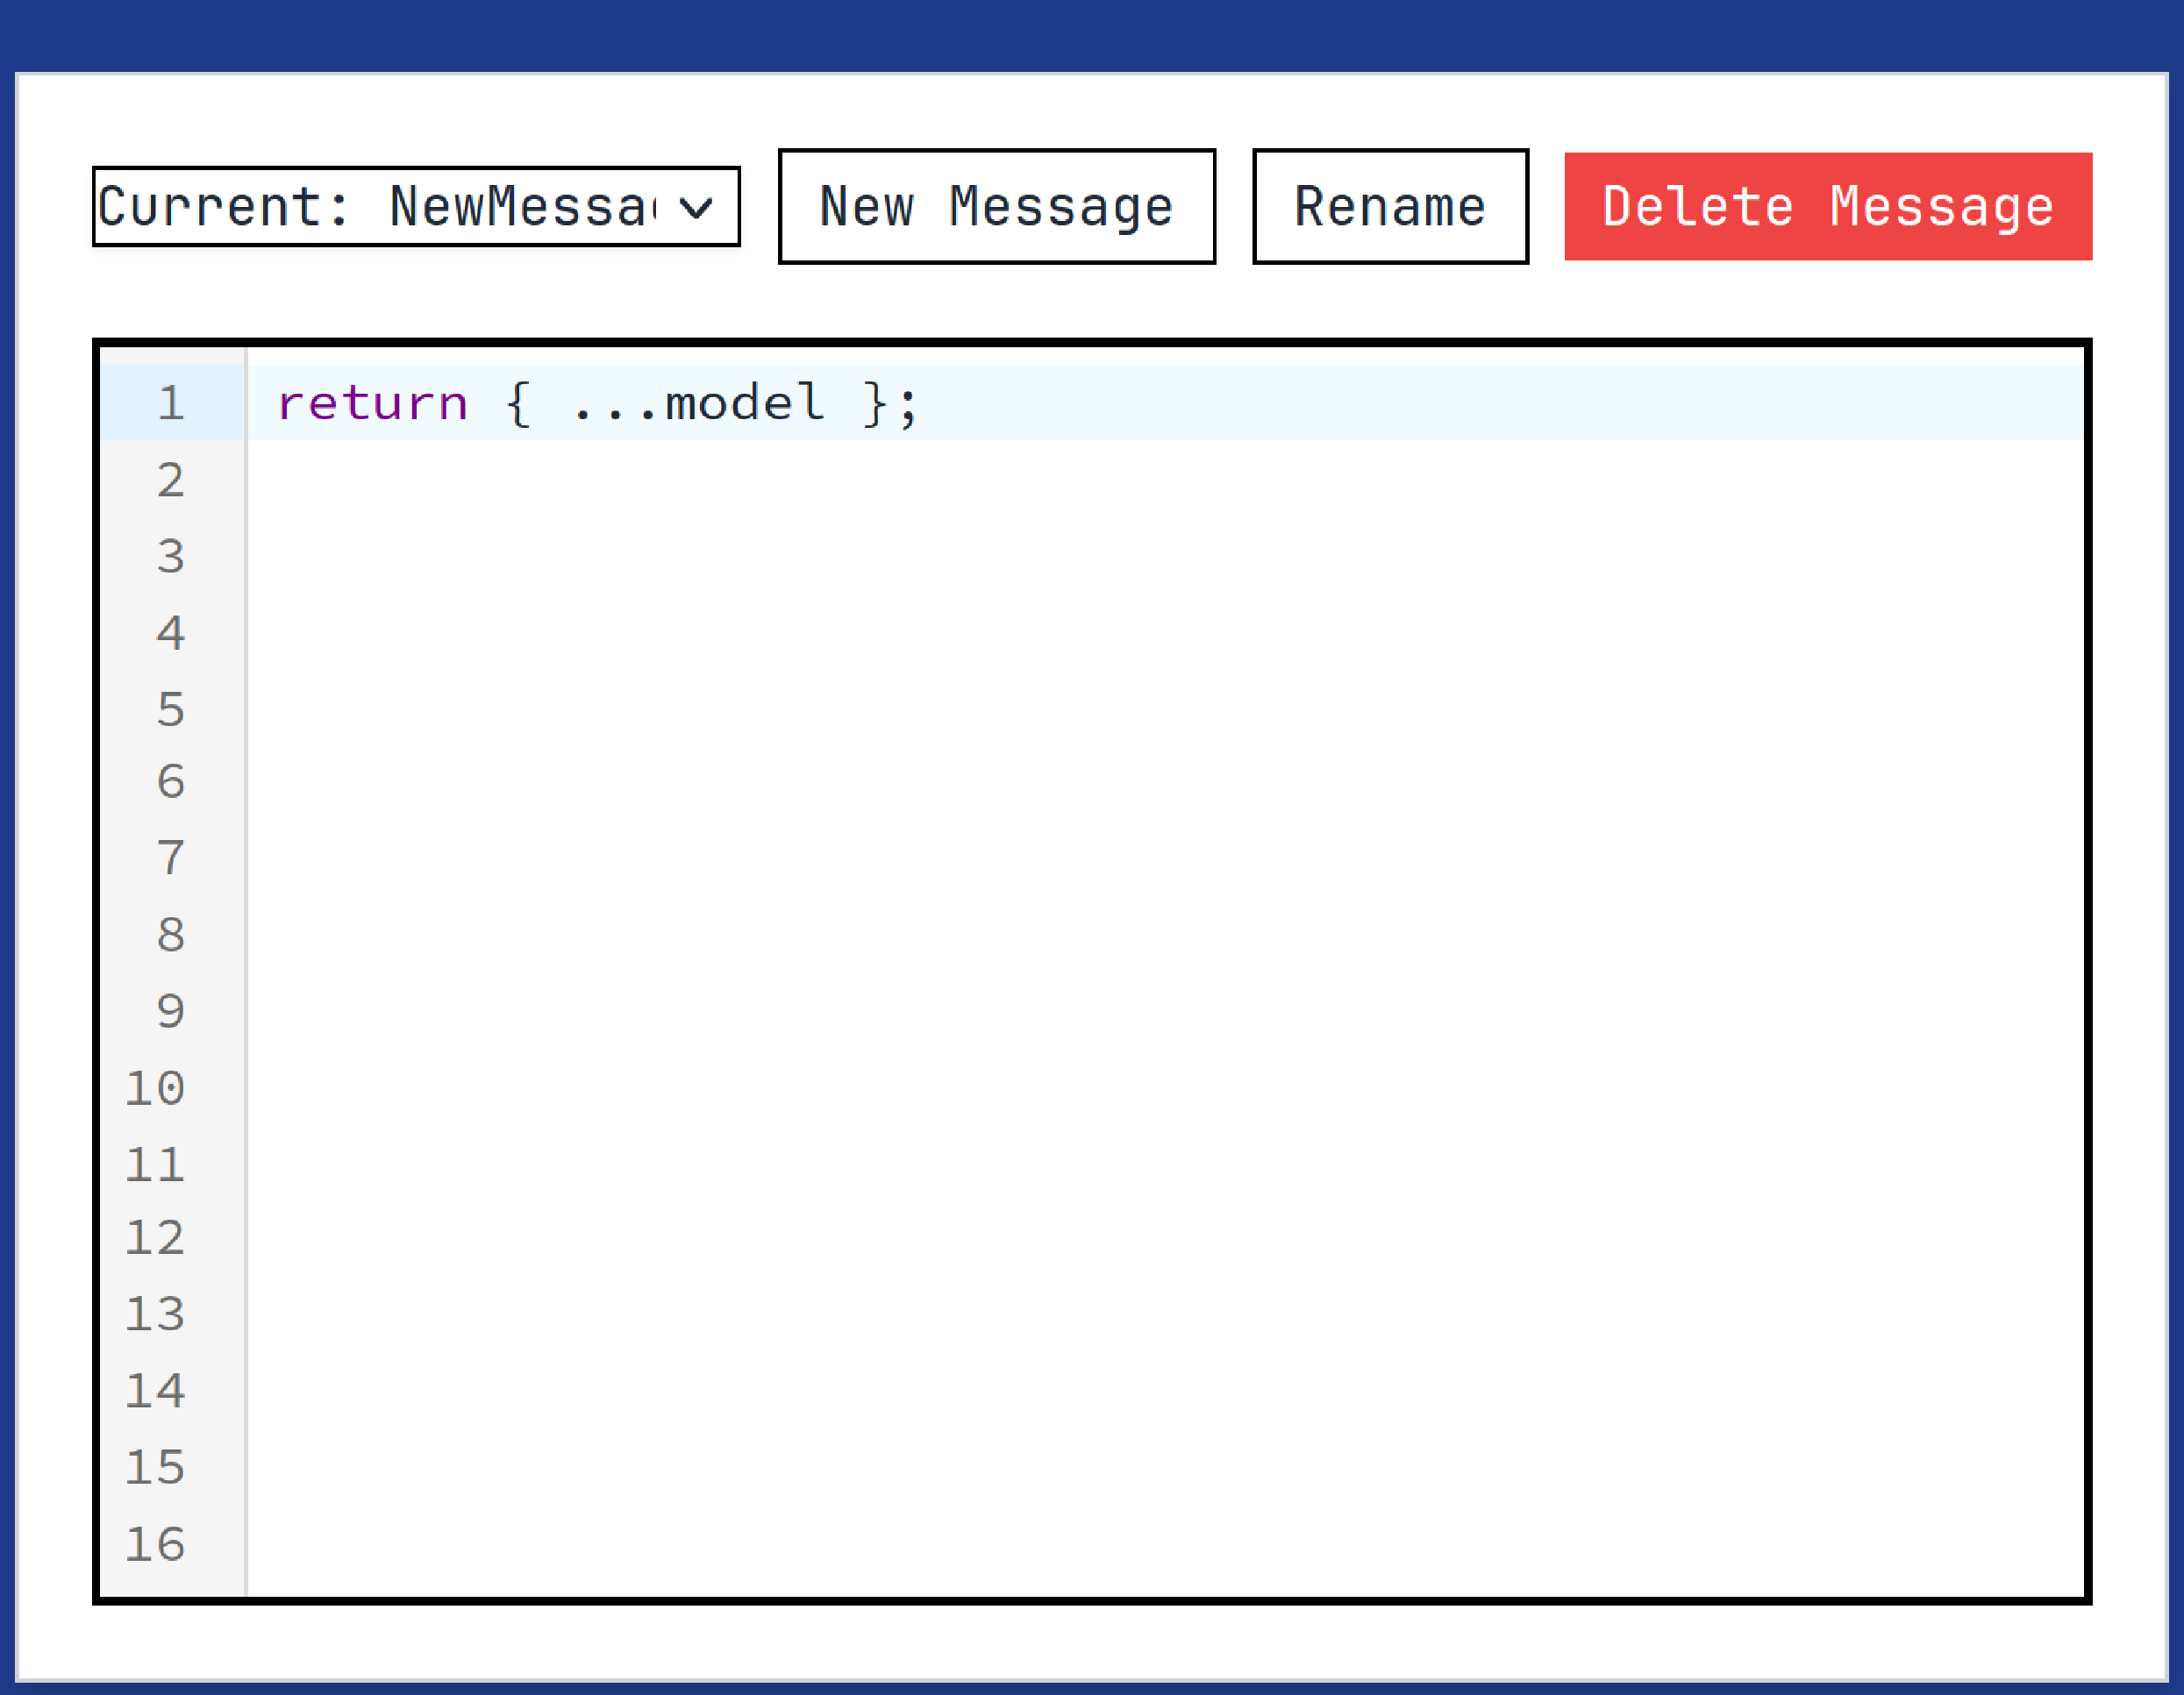
\includegraphics[width=0.7\textwidth]{img/message-menu.pdf}
		      \end{center}
		      \caption{The canvas MessageAndUpdateElement.}\label{fig:message-menu}
	      \end{figure}
	\item \textbf{ViewElement:} A resizable element displaying a preview of the created UI elements alongside modification menus described in Chapter\ref{chap:corelogic} for each element. Also serves as a preview window of the running application.
	      \begin{figure}[htbp]
		      \begin{center}
			      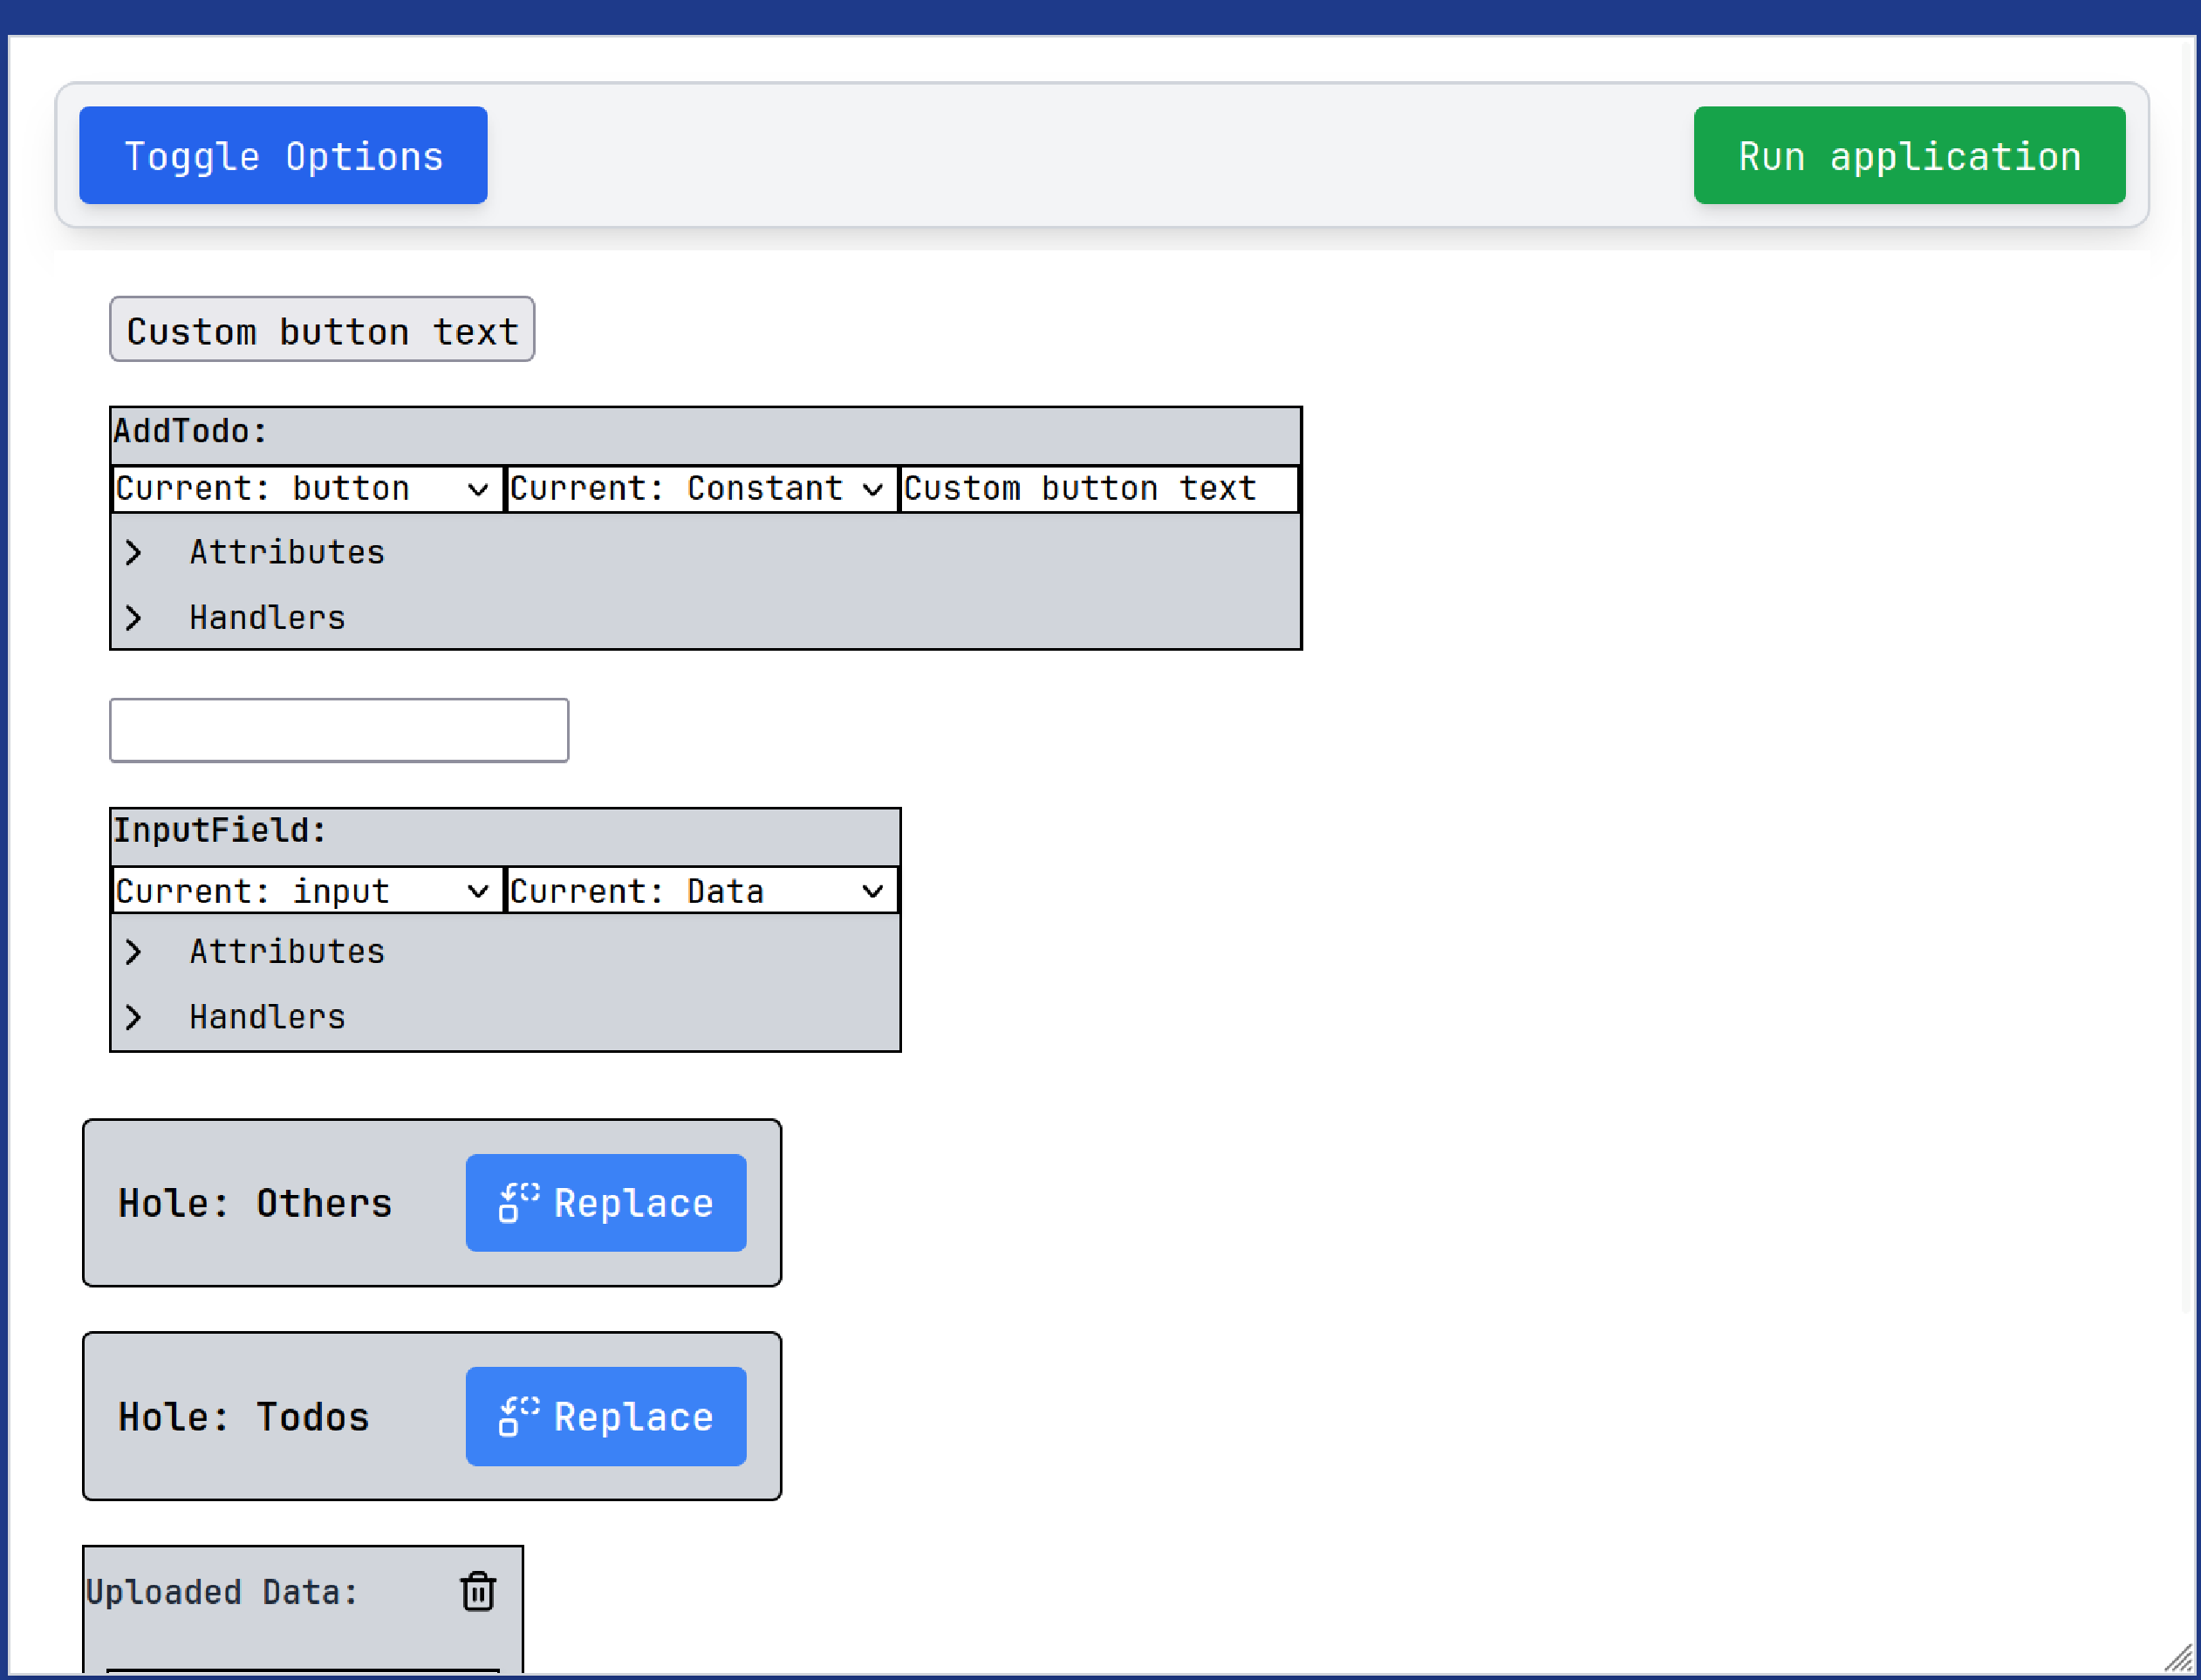
\includegraphics[width=0.7\textwidth]{img/view-menu.pdf}
		      \end{center}
		      \caption{The canvas ViewElement.}\label{fig:view-menu}
	      \end{figure}
\end{itemize}


\medskip
\subsection{Custom Rendering}

To implement the Low-code approach described in Chapter~\ref{chap:design} combined with the Data-driven approach described in Chapter~\ref{chap:corelogic},
we define a \emph{Higher-order} recursive function named \emph{renderingCodeToReactElement}.
This function performs the simultaneous traversal of the \emph{RenderingCode} and JSON ASTs described in Chapter~\ref{chap:corelogic}.
This function provides the main functionality of our implementation and effectively combines the functionality from the \emph{Core logic} module,
with the low-code approach.
It is used by the previously described \emph{ViewElement}.

The function recursively traverses the RenderingCode AST, matching each type of RenderingCode to its appropriate rendering function.
We then define a rendering function for each type of RenderingCode.
Each rendering function combines the RenderingCode structure with the corresponding JSON data to create a preview of the element.
The function also interweaves option menus with the rendered elements, allowing for editing of the rendered structure.
Error handling is implemented throughout the rendering process to handle mismatches between the RenderingCode and JSON structures.

The function takes two arguments, the current RenderingCode node and \emph{RenderingContext}.
The RenderingContext type provides information necessary for correctly rendering the preview of the RenderingCode and the modification menu.
We define the RenderingContext type as seen in Program~\ref{fig:renderingContext}.
\begin{listing}[htpb]
	\begin{lstlisting}
type RenderContext<'Msg> = {
    Options:
        ('Msg -> unit)
            -> RenderingCode
            -> list<int>
            -> string
            -> Map<string, Javascript>
            -> UserMessage list
            -> ReactElement
    Dispatch: 'Msg -> unit
    Json: Json
    Path: int list
    Name: string
    CustomFunctions: Map<string, Javascript>
    ShowOptions: bool
    UserMessages: UserMessage list
}
      \end{lstlisting}
	\caption{The RenderingContext type definition.}\label{fig:renderingContext}
\end{listing}


\clearpage
\subsection{Code generation}

One of our core design principles, as outlined in Chapter~\ref{chap:design},
is the ability to generate a textual representation of the created application.
We define a recursive function named \emph{generateJavaScript} to implement this functionality.
It generates a complete JavaScript application using the \citet{elm-arch}, transforming RenderingCode into client-side JavaScript code.

As the user uploads the JSON data in its text representation to the application, we can directly use it.
We create the \emph{Model} type, equal to the uploaded JSON and representing the application's state.
This then allows us to reference this model and also change the state.

The \emph{view} functions are generated using a recursive function called \emph{generateView}.
This function operates like the \emph{renderingCodeToReactElement} function described in the previous section,
performing a traversal of the RenderingCode ASTs.
For each type of RenderingCode, the function generates the appropriate JavaScript code:
\begin{itemize}
	\item \texttt{HtmlElement} is translated into its corresponding HTML element, attributes, and event handlers.
	\item \texttt{HtmlList} generates Javascript code to dynamically render the list elements, the attributes of the list, and its event handlers.
	\item \texttt{HtmlObject} is translated to its corresponding HTML representation based on the selected \emph{ObjType}, along with its attributes and event handlers.
	\item \texttt{Hole} elements are represented as comments in the generated HTML, maintaining the structure for potential future updates.
\end{itemize}
\noindent A key feature of this function is its ability to automatically populate the generated HTML elements with the corresponding reference to the JSON data,
ensuring that the textual representation accurately reflects the created application's structure and content.
The references to the JSON data are created dynamically by creating a ``path'' of the field names during the traversal, which then accurately reflects the structure of the \emph{Model}.

As the user can create custom \emph{messages}, we generate the \emph{Msg} object, which holds the created messages.
The \emph{update} function is generated as a JavaScript function and takes three arguments, the \emph{Msg}, the event that triggered the dispatching of this message, and the current application's state.
The function consists of a JavaScript \emph{switch statement}, where each case corresponds to a specific message.
The body of the cases is specified by the user and inserted without change.

The \emph{startApplications} function is generated the same way for all applications implemented using the \emph{InterfaceSmith} system.
It sets the model's value to the input data, provides re-rendering functionality, and creates a dispatch function, which calls the \emph{update} function when a specific UI event is triggered.
We see the function along the other parts of the application in Program~\ref{fig:code-generation}.
The result is then inserted into a script HTML element inside an HTML project template.

\begin{listing}[H]
	\begin{lstlisting}
const Msg = {
  MsgExample: "MsgExample",
};

const model = {
  value : 0
};

const update = (msg, event, model) => {
  switch (msg) {
    case Msg.MsgExample:
      return { ...model };
    default:
      return model;
  }
};

const view = (model, dispatch) => `
<div  >
<label  >${model.value}</label>
</div>`;

function startApplication(initialModel, updateFunction, viewFunction) {
  let currentModel = initialModel;
  const render = () => {
    const root = document.getElementById("app");
    root.innerHTML = viewFunction(currentModel, dispatch);
  };
  window.dispatch = (msg, event) => {
    currentModel = updateFunction(msg, event, currentModel);
    render();
  };
  render();
}

startApplication(model, update, view);
	\end{lstlisting}
	\caption{An example Elm-style application generated by the \emph{InterfaceSmith} system.}\label{fig:code-generation}
\end{listing}


\clearpage
\section{Building and Deployment}
\label{sec:build}
Now that we have described the implementation of the \emph{InterfaceSmith} system, we must describe how the application is built and deployed.
As we mentioned in Section~\ref{sec:technologies}, we use the \emph{Build} project provided by the \citet{safestack} template.
The original SAFE stack \emph{Build} project supports building \emph{full-stack} applications written in F\#, and we modified it to remove the support for building
the \emph{Shared} and \emph{Server} projects, as our programming system only consists of a client-side application.
\medskip
\subsection{Build Tools and Libraries}
The SAFE stack \emph{Build} project employs different specialized tools to make building F\# application easier.
The two main tools used by the \emph{Build} project are the following:
\begin{itemize}
	\item \textbf{FAKE (F\# Make):} A build automation tool for projects written in F\#, used to define build targets and their individual build steps.
	\item \textbf{Vite:} A web development tool for building JavaScript client-side applications, which provides a development server environment with Hot Module Replacement capability.
\end{itemize}


The pre-requisites are needed to build the application:
\begin{itemize}
	\item \textbf{.NET Core SDK 8}
	\item \textbf{Node 20}
\end{itemize}

\medskip
\subsection{Build targets}
The \emph{Build} project provides multiple different build targets.
Each provides a different build result and comprises a different sequence of build steps.

The \emph{Build} project defines the following targets:
\begin{itemize}
	\item \textbf{Run:} Configuration for running a local development server with HMR capabilities.
	      Uses the Fable compiler to compile the source code into JavaScript and uses Vite to run the development server.
	\item \textbf{Bundle:} Target used for bundling of the application for deployment.
	      Uses the Fable compiler to compile the source code into JavaScript and uses Vite to
	      bundle and optimize the application assets, including the JavaScript program, CSS, and static files.
	\item \textbf{RunTests:} Configuration for running the unit tests.
	\item \textbf{Format:} Uses the \emph{Fantomas} F\# code formatter, to format the source code.
\end{itemize}

In order to build a specific target, we use the following command:
\begin{lstlisting}[language=bash]
  dotnet run [Target] 
\end{lstlisting}
It consists of the \emph{dotnet run} command, followed by the name of the target we wish to build.
It is important to mention, that the target names are case-sensitive.
\medskip
\subsection{Deployment}
We provide a deployment solution in a form of a \texttt{Dockerfile}.
To run or deploy the \emph{Data-driven UI} docker image, we must first build it using the following command inside the root of the project:
\begin{lstlisting}[language=bash]
  docker build -t data-driven-ui .  
\end{lstlisting}

After the build process is finished, we can run the docker container by running the following command which starts the docker image and makes the application accessible on port 8080:
\begin{lstlisting}[language=bash]
   docker run -p 8080:80 data-driven-ui  
\end{lstlisting}

\medskip
\section{Testing}
\label{sec:testing}
To ensure that the implemented operations perform as expected, we decided to create a separate project named \emph{Tests}.
We implemented \emph{Unit tests} for various operations from the Core Logic module, such as the \emph{replace} function from the \emph{CoreLogic.Operations.RenderingCode} module, and the code generation capability from the \emph{CoreLogic.Operations.CodeGeneration} module.

We use the testing library named \citet{mocha}, which provides useful tools to implement the testing functionality.
It provides a browser-based testing environment with a graphical user interface displaying the individual test cases and their results.
It also allows composing related \emph{test cases} into \emph{test lists}, improving the readability and maintainability of the tests.

The structure of the individual test cases follows the \emph{Arange Act Assert} (AAA) unit test pattern.
It involves preparing the required data, then performing some operation using this data, and then asserting that the operation has the expected result.
We can see an example test case in Program~\ref{fig:test}.
We can see the name of the test case and its implementation which follows the \emph{AAA} pattern.

\begin{listing}[htbp]
	\caption{An example test case testing the functionality of the \emph{replace} function.}
	\label{fig:test}
	\begin{lstlisting}
testCase "Replace Hole"
  <| fun _ ->
      let original = Hole(Named "placeholder")
      let replacement = HtmlElement(Div, [], Empty, [])
      let result = replace [] replacement original
      Expect.equal result replacement "Should replace Hole at root level"
  \end{lstlisting}
\end{listing}

\clearpage
\section{Summary}

In this chapter, we described the practical implementation of our Data-driven UI programming system,
translating the theoretical concepts and core logic into a functional prototype.
The key points covered in this chapter are:

\begin{itemize}
	\item In Section~\ref{sec:technologies}, we outlined the technologies used in our implementation, including F\#, Fable, React, Elmish, and others.
	      We also discussed alternative technologies considered and our rationale for our choices.

	\item In Section~\ref{sec:appArch}, we presented the system architecture,
	      detailing the modular structure of our implementation.
	      We described the Core Logic and Editor modules, explaining how they interact and their respective responsibilities.

	\item In Section~\ref{sec:features}, we explored the main features of our system, focusing on:
	      \begin{itemize}
		      \item The user interface, which combines an application-level Elm architecture with component-level Elmish architecture for more complex elements.
		      \item The custom rendering system, which implements the low-code and data-driven approaches through the \texttt{renderingCodeToReactElement} function.
		      \item The code generation capability, which translates our internal representations into HTML and JavaScript.
	      \end{itemize}

	\item In Section~\ref{sec:build}, we described the build and deployment process, detailing the tools used and the available build targets.

	\item In Section~\ref{sec:testing}, we outlined our testing approach, explaining how we use unit tests to verify the correctness of our core operations.
\end{itemize}






